\begin{figure}[H]
    \centering
    \def\angle{0}
    \def\radius{3}
    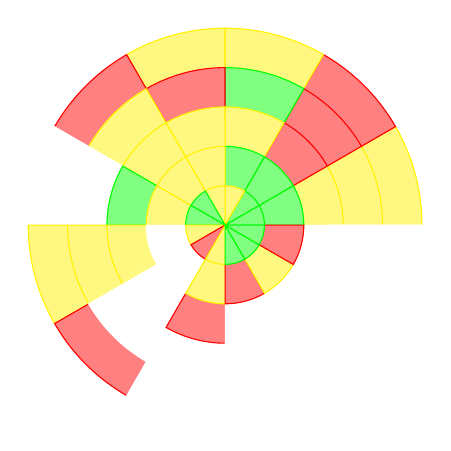
\begin{tikzpicture}[nodes = {font=\sffamily}]
      \foreach \color in {
            yellow,
            red,
            yellow,
            white,
            red,
            yellow,
            white,
            yellow,
            white,
            white,
            red,
            red,
        } {
        \ifx\color\empty\else
            \draw[fill={\color!50},draw={\color}] (0,0) -- (\angle:\radius)
              arc (\angle:\angle+30:\radius) -- cycle;
            \pgfmathparse{\angle+30}
            \xdef\angle{\pgfmathresult}
        \fi
        };
        \xdef\radius{2.5}
        \foreach \color in {
            yellow,
            red,
            yellow,
            yellow,
            red,
            white,
            yellow,
            red,
            white,
            white,
            white,
            white,
        } {
        \ifx\color\empty\else
            \draw[fill={\color!50},draw={\color}] (0,0) -- (\angle:\radius)
              arc (\angle:\angle+30:\radius) -- cycle;
            \pgfmathparse{\angle+30}
            \xdef\angle{\pgfmathresult}
        \fi
        };
        \xdef\radius{2}
        \foreach \color in {
            yellow,
            red,
            green,
            red,
            yellow,
            white,
            yellow,
            white,
            white,
            white,
            white,
            white,
        } {
        \ifx\color\empty\else
            \draw[fill={\color!50},draw={\color}] (0,0) -- (\angle:\radius)
              arc (\angle:\angle+30:\radius) -- cycle;
            \pgfmathparse{\angle+30}
            \xdef\angle{\pgfmathresult}
        \fi
        };
        \xdef\radius{1.5}
        \foreach \color in {
            yellow,
            red,
            yellow,
            yellow,
            yellow,
            green,
            yellow,
            white,
            red,
            white,
            white,
            white,
        } {
        \ifx\color\empty\else
            \draw[fill={\color!50},draw={\color}] (0,0) -- (\angle:\radius)
              arc (\angle:\angle+30:\radius) -- cycle;
            \pgfmathparse{\angle+30}
            \xdef\angle{\pgfmathresult}
        \fi
        };
        \xdef\radius{1}
        \foreach \color in {
            green,
            green,
            green,
            yellow,
            yellow,
            yellow,
            white,
            white,
            yellow,
            red,
            yellow,
            red,
        } {
        \ifx\color\empty\else
            \draw[fill={\color!50},draw={\color}] (0,0) -- (\angle:\radius)
              arc (\angle:\angle+30:\radius) -- cycle;
            \pgfmathparse{\angle+30}
            \xdef\angle{\pgfmathresult}
        \fi
        };
        \xdef\radius{0.5}
        \foreach \color in {
            green,
            green,
            yellow,
            yellow,
            green,
            green,
            yellow,
            red,
            yellow,
            green,
            green,
            green,
        } {
        \ifx\color\empty\else
            \draw[fill={\color!50},draw={\color}] (0,0) -- (\angle:\radius)
              arc (\angle:\angle+30:\radius) -- cycle;
            \pgfmathparse{\angle+30}
            \xdef\angle{\pgfmathresult}
        \fi
        };
    \end{tikzpicture}
\caption{Typical gateway coverage\cite{lorajambalaya}\label{fig:coverage}}
\begin{tabular}{r@{: }l r@{: }l}

\begin{tikzpicture}\draw[fill=green,line width=1pt]  circle(1ex);\end{tikzpicture} & Good\ Connection & 
\begin{tikzpicture}\draw[fill=yellow,line width=1pt]  circle(1ex);\end{tikzpicture} & Intermediate\ Connection\\

\begin{tikzpicture}\draw[fill=red,line width=1pt]  circle(1ex);\end{tikzpicture} & Bad\ Connection & 
\begin{tikzpicture}\draw[fill=white,line width=1pt]  circle(1ex);\end{tikzpicture} & No\ Connection 
\end{tabular}
\end{figure}


